\documentclass[UTF8, a4paper, 11pt]{article}
\usepackage{diagbox}
\usepackage{subfigure}
\usepackage[UTF8, scheme=plain]{ctex}
\usepackage{fontspec}
\usepackage{float}
\usepackage{amsmath}
\newtheorem{myDef}{Definition}
\usepackage{graphicx}
\usepackage{geometry}
\usepackage{listings}
\usepackage{xcolor}
\usepackage{caption}
\geometry{scale=0.8}
\linespread{1.5}
\usepackage{hyperref}
\usepackage{color}
\usepackage{fontspec}
\usepackage{enumitem}
\usepackage[linesnumbered,boxed]{algorithm2e}    
\usepackage{xeCJK}
\usepackage{indentfirst} 
\graphicspath{{Pics/}} 	% 在于.tex同级的目录下创建名为pic的文件夹,存放图片


\setlength{\parindent}{2em}

\lstset{
    language={python},
    frame=shadowbox,
    breaklines=true,
    numbers=left,
    backgroundcolor=\color[RGB]{245,245,244},
    rulesepcolor=\color{red!20!green!20!blue!20},
    numberstyle={\color[RGB]{0,192,192}\tiny},
    basicstyle=\footnotesize \fontspec{Source Code Pro}
}
\setenumerate[1]{itemsep=0pt,partopsep=0pt,parsep=\parskip,topsep=0pt}
\setitemize[1]{itemsep=0pt,partopsep=0pt,parsep=\parskip,topsep=0pt}
\setdescription{itemsep=0pt,partopsep=0pt,parsep=\parskip,topsep=0pt}


\title{	
\normalfont \normalsize
\textsc{School of Data and Computer Science, Sun Yat-sen University} \\ [25pt] %textsc small capital letters
\rule{\textwidth}{0.5pt} \\[0.4cm] % Thin top horizontal rule
\huge SVM\\ % The assignment title
\rule{\textwidth}{2pt} \\[0.5cm] % Thick bottom horizontal rule
\author{18308045 谷正阳}
\date{\normalsize\today}
}

\begin{document}
\maketitle
\tableofcontents
\newpage
\section{Preprocessing}
\subsection{Feature extraction: TF-IDF}
Tf means term-frequency while tf-idf means term-frequency times inverse document-frequency.
The term-frequency helps to scale down the impact of very long documents, while the inverse document-frequency is to scale down the impact of tokens that occur very frequently in a given corpus and that are hence empirically less informative than features that occur in a small fraction of the training corpus.
The formula that is used to compute the $tf-idf$ for a term $t$ of a document $d$ in a document set is
$$tf-idf(t,d)=tf(t,d)idf(t)$$
, and the $idf$ is computed as
$$idf(t)=\log(\frac n{df(t)+1})$$
, where $tf$ is the term-frequency in one classification, $n$ is the total number of documents in the document set and $df(t)$ is the document frequency of t.
\begin{figure}[H]
    \centering
    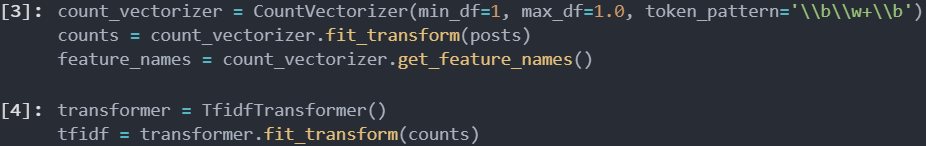
\includegraphics[width=0.8\textwidth]{tfidf.png}
\end{figure}
\subsection{Feature selection: chi2}
Since the number of features is too large, the time and space complexity can be very high and the lack of training set can lead to overfitting.
Therefore, I use the chi2 score to select $K$ best features.
\begin{figure}[H]
    \centering
    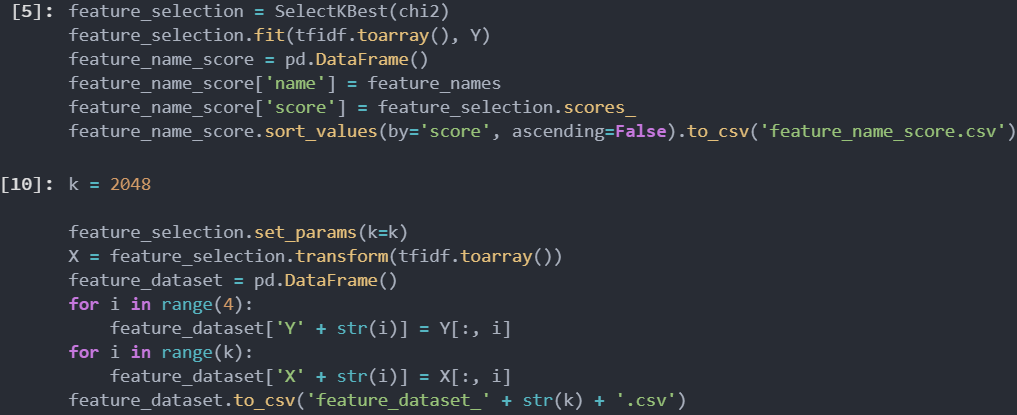
\includegraphics[width=0.8\textwidth]{chi2.png}
\end{figure}
\subsection{Dimensionality reduction: PCA}
PCA is a way of linear dimensionality reduction, which uses Singular Value Decomposition of the data to project it to a lower dimensional space.
The basic idea of PCA is to minimize the recounstruction error and meanwhile to ensure that the projections of all points are separated as far as possible.
\begin{figure}[H]
    \centering
    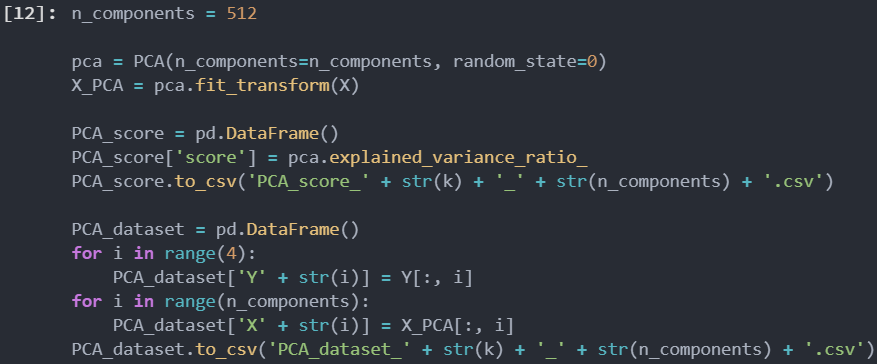
\includegraphics[width=0.8\textwidth]{pca.png}
\end{figure}
\subsection{Representation of outputs}
The problem is to classify people into 16 personality types across 4 axis based on their posts.
Therefore, a 4-output one-hot vector is a good representation of personality types.
\begin{figure}[H]
    \centering
    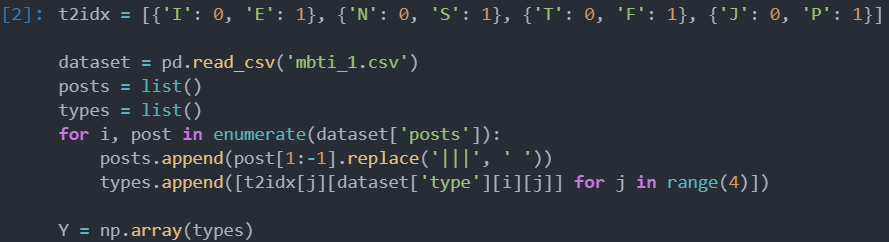
\includegraphics[width=0.8\textwidth]{4-outputs.png}
\end{figure}
\section{Classification}
I change the number of selected features, the number of features after PCA, and generate several csv files storing datasets and scores separately.
Using these datasets, I test several hyperparameters' impact on the model.
\subsection{The number of selected features}
Firstly, I test the impact of different number of selected features.
\begin{figure}[H]
    \centering
    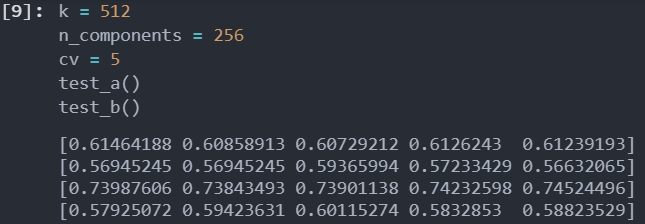
\includegraphics[width=0.8\textwidth]{k.png}
\end{figure}
k stands for the number of selected features, n\_components stands for the number of features after PCA, cv represents cross-validation splitter, and the four lines of outputs respectively represent training scores before PCA, testing scores before PCA, training scores after PCA and testing scores after PCA.
The first 2 lines of outputs are what we should consider in this section.
\begin{table}[H]
    \center
\begin{tabular}{|l|l|l|}
\hline
k    & Average training score & Average testing score \\ \hline
512  & 0.611107872            & 0.5742439559999999    \\ \hline
1024 & 0.6302454880000001     & 0.577125136           \\ \hline
2048 & 0.651083652            & 0.580121922           \\ \hline
4096 & 0.6613730180000001     & 0.577124804           \\ \hline
8192 & 0.688119534            & 0.57643296            \\ \hline
\end{tabular}
\end{table}
When k is larger than 2048, overfitting apparently happens.
\subsection{The number of features after PCA}
Then I set the k as 2048 and test the impact of different number of features after PCA.
\begin{figure}[H]
    \centering
    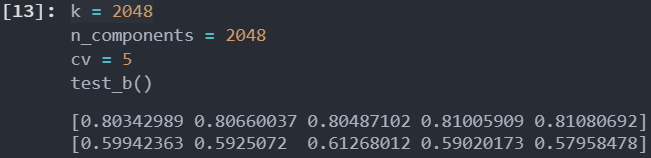
\includegraphics[width=0.8\textwidth]{n_components.png}
\end{figure}
Except for the average training scores and average testing scroes, I also add the summation of percentage of variance which is stored in PCA\_k\_n\_components\_score.csv.
\begin{table}[H]
    \center
\begin{tabular}{|l|l|l|l|}
\hline
n\_components & Average training score & Average testing score & Percentage of variance \\ \hline
512          & 0.7893992540000001     & 0.595341118           & 0.956029               \\ \hline
1024         & 0.802570794            & 0.596262778           & 0.993766               \\ \hline
2048         & 0.8071534579999999     & 0.5948794920000001    & 1                      \\ \hline
\end{tabular}
\end{table}
It is shown that 1024 is the best n\_components.
\subsection{Regularization parameter for l2 penalty}
There is also a regularization parameter in SVM implemented by sklearn, so I test it's impact on the model.
\begin{figure}[H]
    \centering
    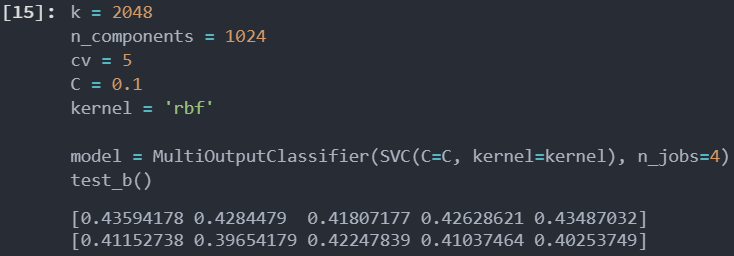
\includegraphics[width=0.8\textwidth]{C.png}
\end{figure}
C represents the regularization parameter and kernel stands for kernel function used in SVM model.
\begin{table}[H]
    \center
\begin{tabular}{|l|l|l|}
\hline
C   & Average training score & Average testing score \\ \hline
0.1 & 0.42872359600000004    & 0.4086919379999999    \\ \hline
1   & 0.802570794            & 0.596262778           \\ \hline
1.5 & 0.860819626            & 0.6032962700000001    \\ \hline
1.7 & 0.876585084            & 0.605140584           \\ \hline
1.8 & 0.8846551619999999     & 0.6052557920000001    \\ \hline
1.9 & 0.89180294             & 0.605140454           \\ \hline
2   & 0.899181334            & 0.60444881            \\ \hline
2.5 & 0.925812676            & 0.603065392           \\ \hline
3   & 0.944056904            & 0.6015663659999999    \\ \hline
5   & 0.982072868            & 0.596263774           \\ \hline
10  & 0.998443634            & 0.5880782040000001    \\ \hline
\end{tabular}
\end{table}
It is shown that 1.8 is the best C.
\subsection{Kernel function}
Finally I test the impact of kernel function on the model.
\begin{figure}[H]
    \centering
    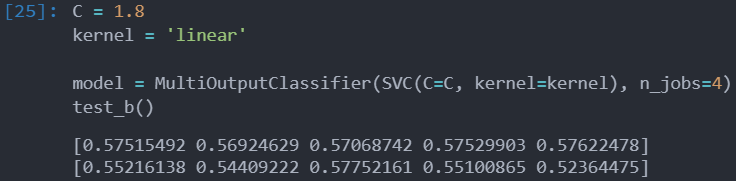
\includegraphics[width=0.8\textwidth]{kernel.png}
\end{figure}
\begin{table}[H]
    \center
\begin{tabular}{|l|l|l|}
\hline
kernel  & Average training score & Average testing score \\ \hline
linear  & 0.573322488            & 0.549685722           \\ \hline
poly    & 0.785191332            & 0.45134602399999996   \\ \hline
rbf     & 0.8846551619999999     & 0.6052557920000001    \\ \hline
sigmoid & 0.368255656            & 0.34966464999999997   \\ \hline
\end{tabular}
\end{table}
It is shown that rbf is the best kernel.
\section{Conclusions}
There are some aspects that can be improved.
For instance, the CountVectorizer can filter out words that appear frequently or rarely by setting max\_df and min\_df.
And kernel functions can be also used in PCA.
Additionally, there are lots of other hyperparameters of SVM which I just use the default value in this experiment.
%\clearpage
%\bibliography{E:/Papers/LiuLab}
%\bibliographystyle{apalike}
\end{document}
%%% Local Variables:
%%% mode: latex
%%% TeX-master: t
%%% End:
